\documentclass{article}
\usepackage{graphicx,float}
\usepackage{listings}
\usepackage{xcolor}
\usepackage{amsmath}
\usepackage{geometry}
\geometry{left=2.0cm,right=2.0cm,top=2.5cm,bottom=2.5cm}

\lstset{numbers=left,
numberstyle=\tiny,
keywordstyle=\color{blue}, commentstyle=\color[cmyk]{1,0,1,0},
frame=null,
%rulesepcolor=\color{red!20!green!20!blue!20},
basicstyle=\ttfamily\small,
xleftmargin=2em,
xrightmargin=2em,
aboveskip=1em,
showspaces=false
}

\author{Yifan Zhao}
\title{Automatical Learning and Data Mining\\HW4 Report}
\begin{document}
 \maketitle
 \section{Description}
 The data set is the same as the second task described in the homework text. We downloaded about 1300 stocks' per minute price sequences during a 20-day period from google finance websites. Then select those who have more than 5000 cases(Some stocks may miss some cases for delisted). Then we have 757 stocks left. We chose two of them as the target stocks. And decide the different classes according to the up and down of these two stocks:\\1: up up;\\2: up down;\\3: down up;\\3: down down.\\Then the number of descriptors is 755. The number of cases is 5000. The number of classes is 4. All descriptors are real and continuous. Expected outputs are 4-dimension 0-1 vectors valued 1 if and only if the index is equal to the correct class index, otherwise, equal to 0. The training set has 4000 cases, the test set has 1000 cases. Before separate the training set and the test set, we shuffle the whole data set in order to remove the influence of chronical trend.
 \section{Architecture of Auto-encoder}
 \subsection{}We construct the auto-encoder based on the MLP paradigm. The auto-encoder has three layers: \[INPUT\rightarrow HIDDEN\rightarrow OUTPUT\]
 where INPUT has the same size as OUTPUT, i.e., the number of descriptors.
 \subsection{PCA of Original Data}Before computing the correlation matrix of the data, we do following manipulations for each descriptor: Subtract its median(or mean) and divide it with its standard deviation. Subtracting median instead of mean could make the data unbiased because of the definition of median, so we choose median here. After performing the PCA, the 3 cut-off numbers of eigenvalues are as follows :\\R1=50\%: 5\\R2=75\%: 30\\R3=90\%: 91. \\So the sizes of auto-encoder's hidden layer are h1=5, h2=30, h3=91.\\
 The graphs of eigenvalues and their cumulative ratios are as follows:
  \begin{figure}[H]
  \centering
  % Requires \usepackage{graphicx}
  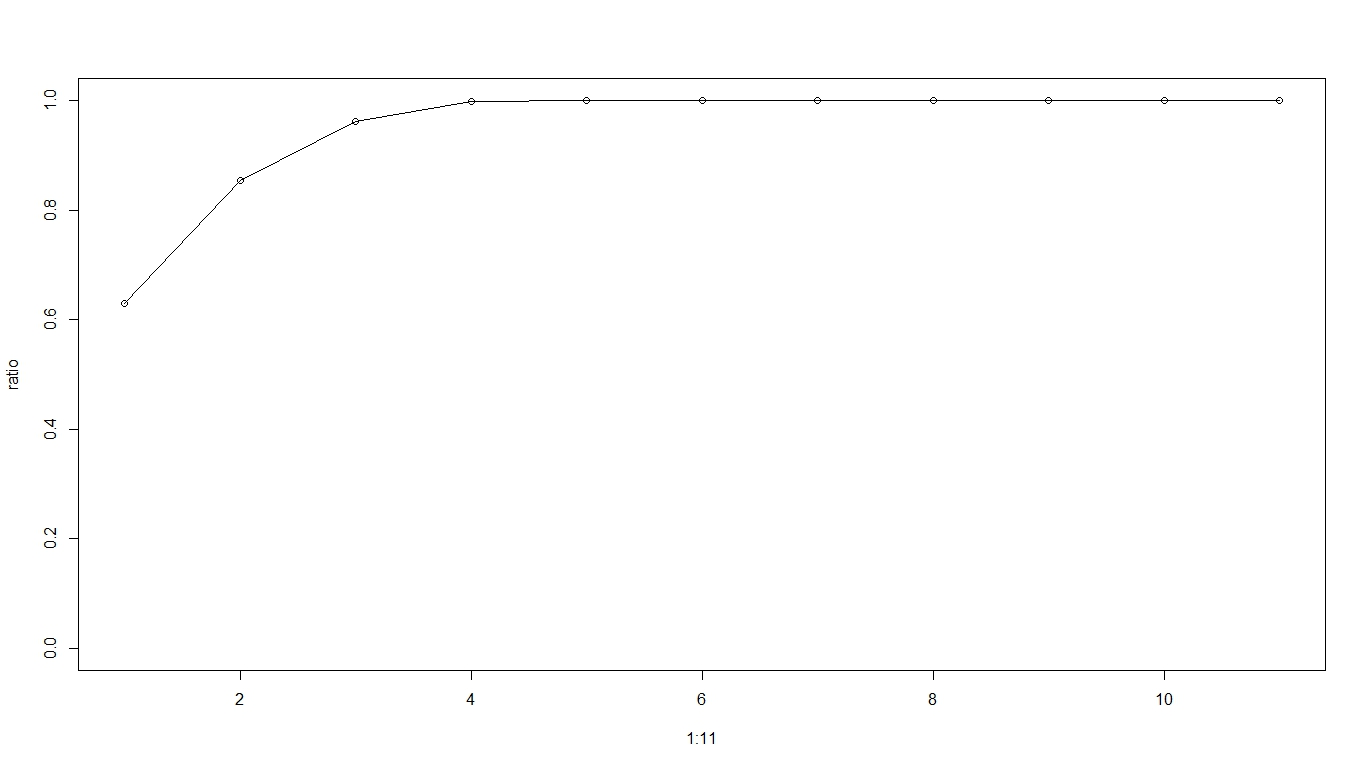
\includegraphics[width=0.75\textwidth]{ratio.jpg}
  \caption{Ratio}\label{}
  \end{figure}
  \begin{figure}[H]
  \centering
  % Requires \usepackage{graphicx}
  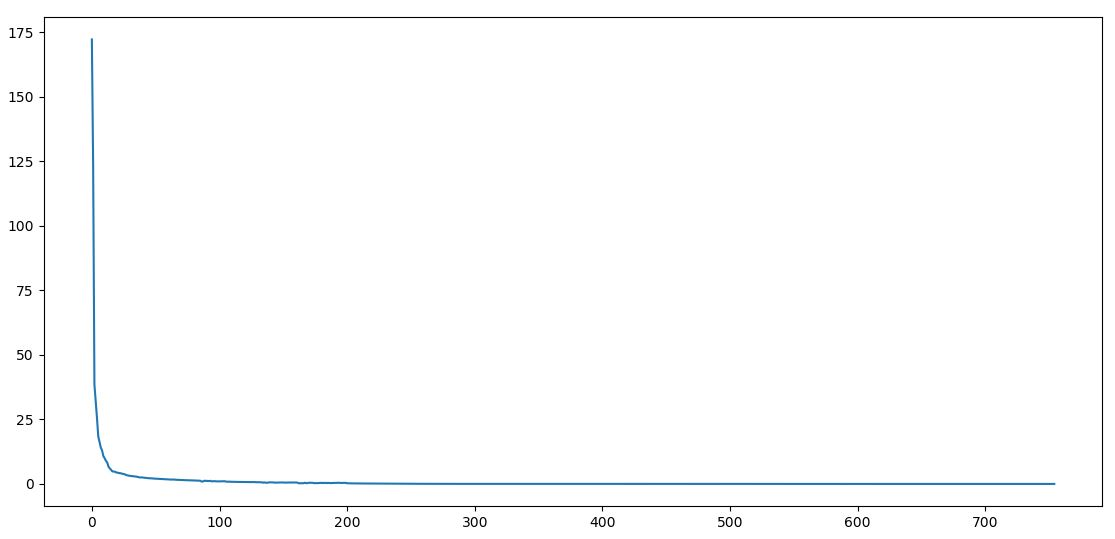
\includegraphics[width=0.75\textwidth]{fracs.jpg}
  \caption{Eigenvalues}\label{}
  \end{figure}
 \subsection{Pretreatment of Original Data}We use the sigmoid response function. Since we have already subtracted the median and divided with standard deviation of the data. And the main non-linear part of sigmoid function is in (-6,6), we do not subtract the minimum of the data, nor divide with the range(maximum minus minimum). The nonlinearity of sigmoid function could be better developed.
 \section{Automatic Learning for 3 AEs}
 \subsection{Software Options}
 We use tensorflow as the software for automatic learning. There are two usual tools for minimizing the MSE on the training set with validation on the test set, ADAM optimizer(function in tensorflow: tf.train.AdamOptimizer) and Gradient Descent optimizer(function in tensorflow: tf.train.GradientDescentOptimizer). The former is a specialized gradient descent optimizer for classification tasks, and the latter is the generic gradient descent optimizer. So we use Graient Descent optimizer in the auto-encoders.\\
 With tensorflow, we could generate various distributed including but not limited to normal distributed tensors for initialization of the wights and assign parameters like means and standard deviations to specify the initialization. One of the appropriate specifications we found is that mean equals to 0.1 and standard deviation equals to 0.01. \\
For batch learning, we use the function np.random.choice in Python package numpy to obtain a batch. This function returns a random sample from the population with a given size. The current tested appropriate batch size is around 100.\\
For the learning rate, we assign a learning rate variable valued $\frac{\epsilon}{n}$to control the step size of gradient, where n the current number of global learning steps or epochs(the latter is better according to several tests).\\
The stopping criterion of learning is when the norm of gradient is smaller than a given level: e.g., 0.03.
For intermediary outputs to monitor learning quality, we compute and print the learning loss per 10 batches. The loss is defined by the mean squared error between reconstructed data and the original input data out of the whole batch.\\
\subsection{RMSE, $\Delta W$, Gradient}
The computation of RMSE, $\Delta W$ and gradient is similar to ordinary MLPs. RMSE is just the square root of MSE, it can be computed by the function tf.sqrt, then normalize it with its dimension. For the $||\Delta W||$, we first compute the norm of the difference of weights and biases of each layer separately. Then we add the squared norms together and normalize it with its dimension. In this way we could avoid to manipulate the matrices of weights and biases, which are pretty complicated. The computation of gradient could be easier after we have the weights' difference, just divide it with the learning rate and normalize it with its dimension.\\
Then we could plot the three curves:
  \begin{figure}[H]
  \centering
  % Requires \usepackage{graphicx}
  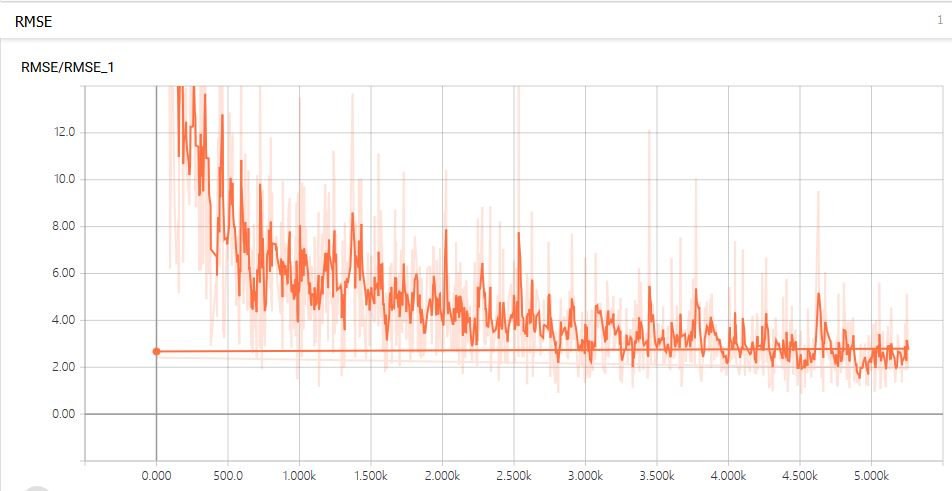
\includegraphics[width=0.75\textwidth]{RMSE.jpg}
  \caption{RMSE}\label{}
  \end{figure}
  \begin{figure}[H]
  \centering
  % Requires \usepackage{graphicx}
  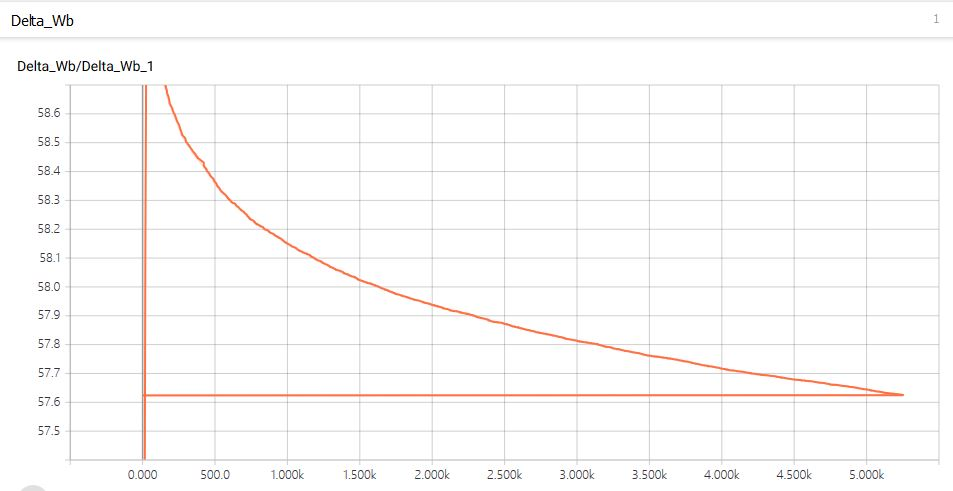
\includegraphics[width=0.75\textwidth]{DeltaWb.jpg}
  \caption{$||\Delta W||$}\label{}
  \end{figure}
  \begin{figure}[H]
  \centering
  % Requires \usepackage{graphicx}
  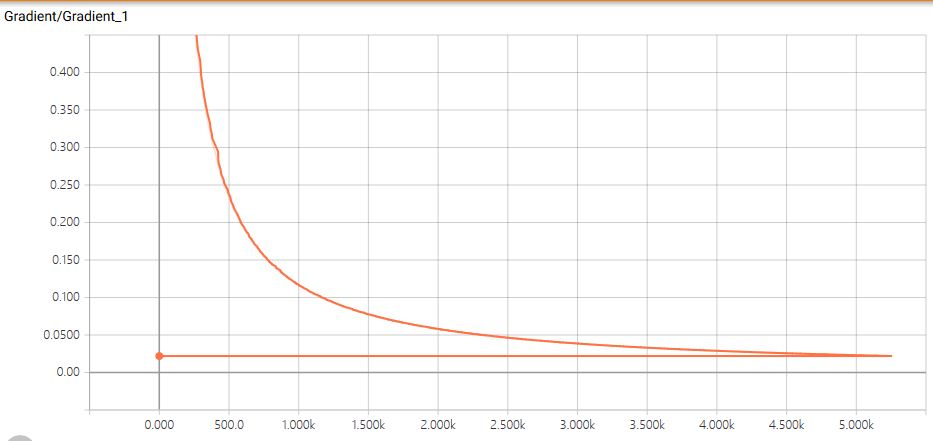
\includegraphics[width=0.75\textwidth]{Gradient.jpg}
  \caption{Gradient}\label{}
  \end{figure}
  As we could see,all three curves decline in an exponential shape as the global steps grow. The fluctuation of RMSE is the greatest among these three curves. The declination of gradient is relatively insignificant comparing with the other two. The learning rate influences the gradient a lot. Therefore, we increased the number of epochs in order to guarantee the auto-encoder converge sufficiently.
  \subsection{Global Performance}
  Here is the graph of two GRMSEs on the same plot.
  \begin{figure}[H]
  \centering
  % Requires \usepackage{graphicx}
  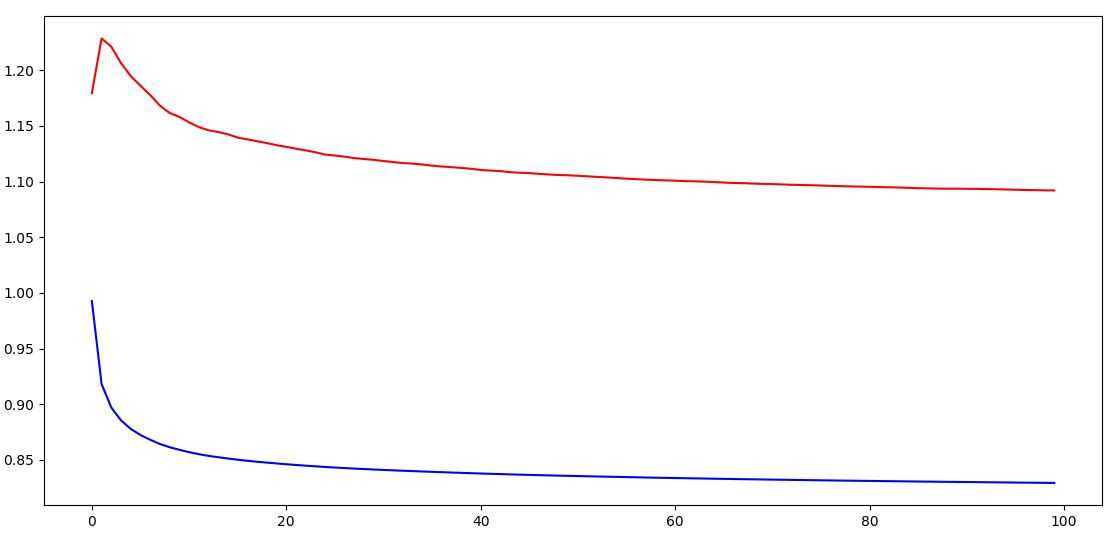
\includegraphics[width=0.75\textwidth]{GRMSE.jpg}
  \caption{GRMSE}\label{}
  \end{figure}
  The blue one represents the training set, the red one represents the test set. As we could see from the graph, the performances on both set are improving as the number of epochs grows. The GRMSE on the test set is slightly greater than that on the training set, yet still comparable.
  \subsection{Performances of Three AEs}
  Since we have 3 different auto-encoders with hidden layer dimensions 5, 30 and 91, we perform several runs of each auto-encoder. The best result is from the 91-dimensional one with batch loss(MSE) converges to 0.06. Obviously, the first two dimensions are too small for reconstructing data with 755 dimensions. Additionally, 91 is a relatively successful compression of data compared with 755. So we select the third auto-encoder as the best.
  \section{Activity Analysis of Hidden Layer}
  \subsection{PCA of Hidden Layer}
  After the training, we save the terminal values of weights and biases. Then we compute the terminal values of hidden layer on the training set. Then implement PCA for these hidden layer vectors. The number of eigenvalues of 90\% energy for the first auto-encoder is 3, the second is 11 and the third is 26. Here is the scatter graph of the cloud of the third auto-encoder. Since graphs for different auto-encoders are not significantly distinct, so we only display the one of 91 dimensions. Points in different classes have different colors.
  \begin{figure}[H]
  \centering
  % Requires \usepackage{graphicx}
  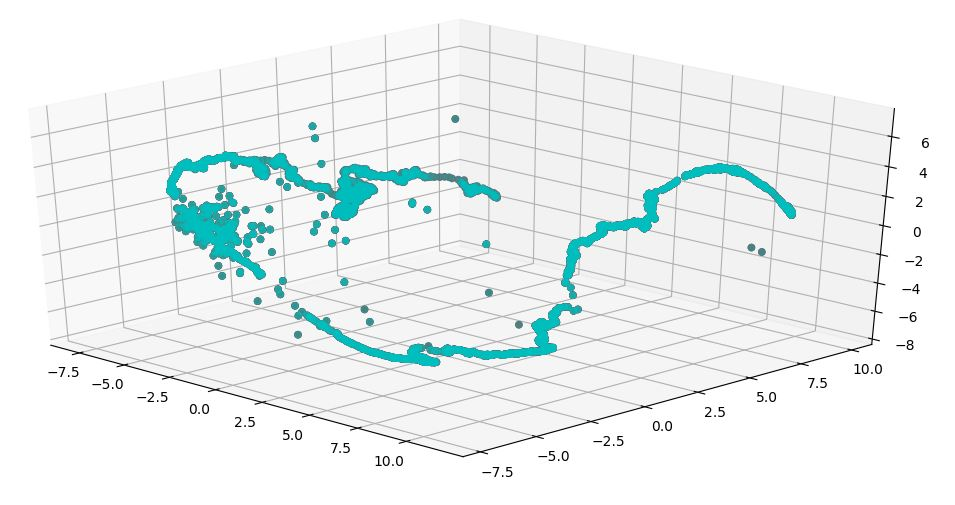
\includegraphics[width=0.75\textwidth]{scatter.jpg}
  \caption{The Cloud of Hidden Layer Vectors}\label{}
  \end{figure}
  As we could see from the scatter, points of different classes have not been separated enough, for auto-encoder is only a pretreatment and simplification of the data. So the implementation of MLP is still necessary.
  \subsection{The Maximum and Activity of Each Node}
  We compute the maximum of each node with following codes. First, we initialize the list variable to store the indices of maximums of each node. Then we find the input such that one specific node attains its maximum by the function np.argmax, it returns the argument(index) such that the input attains its maximum. Then we find the class it belongs to with return value of np.argmax and the array of each input's class index. At last, we count the number of these inputs belonging to each class and return with the list hid\_max\_sum. Here is the list of the number of nodes attributed to each class:\\ \[[14,\ 4,\ 0,\ 73]\]. As we could see, the fourth class is the most active.\\
  The activity of each node is also computed by the following codes. First, we initialize an activity list variable to store the activities. Then for each node, we compute the mean of the node based on the whole set with the function np.mean.
  \begin{lstlisting}[language=Python]
    hid_max=[]
    activity=[]
    class_act=[[],[],[],[]]
    for i in range(h):
        hid_max_index=np.argmax(hidden[:,i])
        hid_max.append(np.argwhere(label[hid_max_index,:]))
        activity.append(np.mean(hidden[:,i]))
        for j in range(n_classes):
            class_act[j].append(np.mean(hidden[label_train_index[j],i]))
    hid_max=np.asarray(hid_max)
    hid_max_sum=[]
    for i in range(n_classes):
        hid_max_sum.append(np.count_nonzero(hid_max==[[i]]))
    print(hid_max_sum)
  \end{lstlisting}
  Then we reorder the activities in increasing order and plot:
  \begin{figure}[H]
  \centering
  % Requires \usepackage{graphicx}
  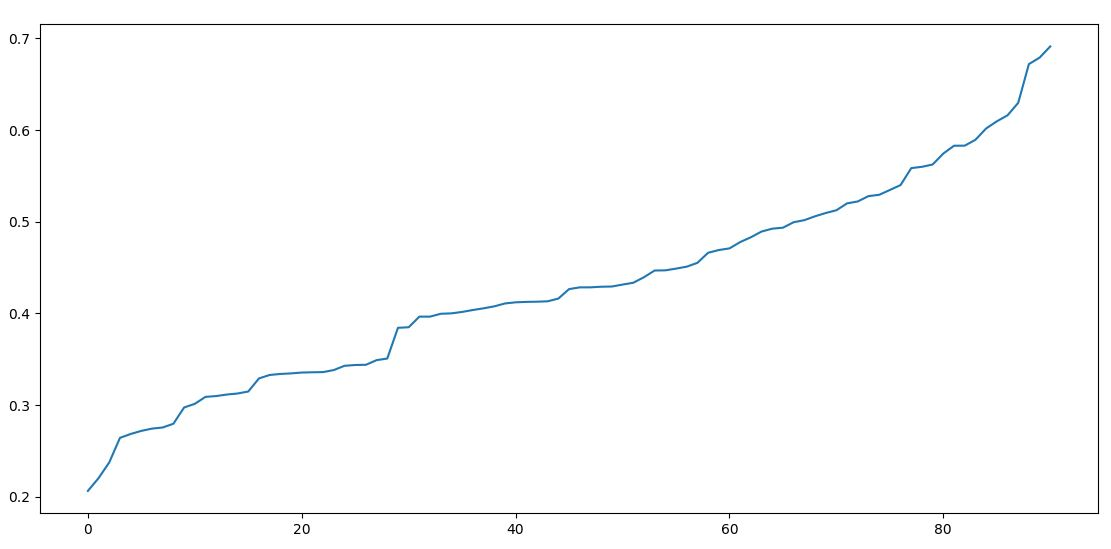
\includegraphics[width=0.75\textwidth]{activity.jpg}
  \caption{Activity}\label{}
  \end{figure}
  As we could see, the activities are all between 0.2 and 0.7, and the number of low activity nodes is small, thus no extreme situations. This is an acceptable result. To identify the nodes with low activities, we first use the function np.argsort to compute the index after reordering Q in increasing order. Then extract those nodes which are in the first 5\% of the array. The 5\% quantile of Q is 4 nodes: 13, 35, 46, 71.\\
  If we remove these nodes, the loss on the whole set will improve from 0.82 to 0.69. Relevant Python codes are as follows. We first initialize the weights variable to store new weights and assign it with all-zero matrix temporarily. Then assign it with the trained terminal weights only in those active nodes indices. Thus we have got the weights matrix with specific rows equal to zero. Then compute the loss with this new matrix.
  \begin{lstlisting}[language=Python]
    act_sort=np.argsort(activity)
    inact_sort=(0.05*len(act_sort))
    act_sort=act_sort[int(inact_sort):]
    W_act=np.zeros([n_des,h])
    b_act=np.zeros([h])
    W_act[:,act_sort]=W[:,act_sort]
    b_act[act_sort]=b[act_sort]
    hid_act=sess.run(tf.sigmoid(np.matmul(train,W_act)+b_act))
    out_act=np.matmul(hid_act,W_out)+b_out
    loss_act = sess.run(tf.losses.mean_squared_error(labels=train, predictions=out_act))
    print("Loss after removing inactive nodes: {0:.2f}".format(loss_act))
  \end{lstlisting}
  Similar analysis for each class could be achieved with following codes:
  \begin{lstlisting}[language=Python]
  for j in range(n_classes):
    class_act[j].append(np.mean(hidden[label_train_index[j],i]))
  \end{lstlisting}
  We compute the activities for each class separately, then we could do the same analysis with the former codes for each class.
  \section{Auto-encoder Insertion in MLP Classifiers}
  \subsection{Architecture of MLP}
  First, we compute the values of AE's hidden layer on the whole set with the terminal weights. Then use these vectors as new inputs. Thus the weigths in the auto-encoder are frozen. According to the PCA of hidden layer, we choose the size of MLP's hidden layer hh=26. After several implementations of the MLP, we modify hh=21 as the best size of hidden layer.
  \subsection{Confusion Matrix}
  We first assign a variable that signifies the class that the cases truly belonged to. Then we compare the class predicted by the output vector with this index variable. Then we compute the ratio of each kind of prediction. Finally after running the session, we could store the results to two matrices and output them.\\
  The training confusion matrix:\\
$[0.7238636363636364,\ 0.003977272727272727,\ 0.006439393939393939\ 0.265719696969697]$\\
$[0.000946969696969697,\ 0.8005681818181818,\ 0.08958333333333333,\ 0.08844696969696969]$\\ 
$[0.0028414472437961733,\ 0.37715476415987875,\ 0.4995264254593673,\ 0.04546315590073877]$\\ 
$[0.005871212121212121,\ 0.11022727272727273,\ 0.014772727272727272,\ 0.8615530303030303]$\\
The test confusion matrix:\\
$[0.7328125,\ 0.005729166666666666,\ 0.004166666666666667,0.25729166666666664]$\\
$[0.00625,\ 0.6572916666666667,\ 0.17447916666666666,\ 0.16145833333333334]$\\
$[0.42239583333333336,\ 0.26666666666666666,\ 0.2864583333333333,\ 0.0234375]$\\ 
$[0.0067708333333333336,\ 0.2140625,\ 0.022916666666666665,\ 0.7473958333333334]$\\
\section{Appendix: Python Codes}
\begin{lstlisting}[language=Python]
import tensorflow as tf
import numpy as np
import pandas as pd
from matplotlib.mlab import PCA
import matplotlib.pyplot as plt
from ops import fc_layer, batch_ae, batch
from mpl_toolkits.mplot3d import Axes3D

count=0
df=pd.read_csv('F:/Files/DataMining/HW4/companylist.csv',
                         usecols=[0],skiprows=[0], header=None)
list=df.values
for i in range(len(list)):
    filename = str(list[i])[2:-2] + '.csv'
    try:
        df = pd.read_csv('F:/Files/DataMining/HW4/data/' + filename,
                 usecols=[2], skiprows=[0, 1, 2, 3, 4, 5, 6], header=None)
    except FileNotFoundError:
        pass
    except pd.io.common.EmptyDataError:
        pass
    if len(df.values)>=5010:
        col=df.values[0:5010]
        col=np.nan_to_num(col)
        m=np.median(col)
        sigma = np.sqrt(np.var(col))
        col=(col-m)/sigma
        if count==0:
            data=col
            count=1
        else:
            data=np.append(data,col,axis=1)

label=np.empty([5000,4])
for j in range(5000):
    if data[j,755]<data[j+10,755]:
        if data[j,756]<data[j+10,756]:
            label[j,:]=[1,0,0,0]
        else:
            label[j, :] = [0, 1, 0, 0]
    else:
        if data[j,756]<data[j+10,756]:
            label[j,:]=[0,0,1,0]
        else:
            label[j, :] = [0, 0, 0, 1]

label_train=label[0:4000,:]
label_test=label[4000:5000,:]
data=data[0:5000,0:755]
data=np.nan_to_num(data)
n_des=data.shape[1]
n_cases=data.shape[0]
data_label=np.append(data,label,axis=1)
train=data[0:4000,:]
test=data[4000:5000,:]
label_train_index=[[],[],[],[],[]]
label_test_index=[[],[],[],[],[]]
for i in range(4):
    label_train_index[i]= label_train[:,i]==1
    label_test_index[i]=label_test[:,i]==1

pca=PCA(data)
co=np.corrcoef(np.transpose(data))
eig=np.linalg.eig(co)

for i in range(n_des):
    if np.sum(eig[0][0:i])>=0.5*np.sum(eig[0]):
        r1=i
        break
for i in range(n_des):
    if np.sum(eig[0][0:i])>=0.75*np.sum(eig[0]):
        r2=i
        break
for i in range(n_des):
    if np.sum(eig[0][0:i])>=0.9*np.sum(eig[0]):
        r3=i
        break
rat=[]
for i in range(755):
    rat.append(np.sum(pca.fracs[0:i]))


epochs=100
test_size=1000
batch_size=100
display_freq=10
h=r3
hh=20
n_classes=4

x = tf.placeholder(tf.float64, shape=[None, n_des], name='X')
y = tf.placeholder(tf.float64, shape=[None, n_des], name='Y')
x1=tf.placeholder(tf.float64, shape=[None, h], name='X1')
z=tf.placeholder(tf.float64, shape=[None, n_classes], name='Z')
learning_rate = tf.placeholder(tf.float64, shape=None, name='epsilon')
W_hid2out_form=tf.Variable(tf.zeros(shape=[h,n_des]),name='W_hid2out_form')
W_in2hid_form=tf.Variable(tf.zeros(shape=[n_des,h]),name='W_in2hid_form')
b_hid2out_form=tf.Variable(tf.zeros(shape=[n_des]),name='b_hid2out_form')
b_in2hid_form=tf.Variable(tf.zeros(shape=[h]),name='b_in2hid_form')
W_hid2out_form=tf.cast(W_hid2out_form,tf.float64)
W_in2hid_form=tf.cast(W_in2hid_form,tf.float64)
b_hid2out_form=tf.cast(b_hid2out_form,tf.float64)
b_in2hid_form=tf.cast(b_in2hid_form,tf.float64)

fc1 = fc_layer(x, h, 'Hidden_layer', use_relu=True)
output_logits = fc_layer(fc1[0], n_des, 'Output_layer', use_relu=False)
fc11 = fc_layer(x1, hh, 'Hidden_layer1', use_relu=True)
output_logits1=fc_layer(fc11[0], n_classes, 'Output_layer1', use_relu=False)

#define the loss defined as mean squared error
with tf.name_scope('MSE'):
    loss = tf.losses.mean_squared_error(labels=y, predictions=output_logits[0])
    tf.summary.scalar('MSE',loss)
loss1 = tf.losses.mean_squared_error(labels=z, predictions=output_logits1[0])
#compute the root MSE
with tf.name_scope('RMSE'):
    rmse=tf.sqrt(loss,name='RMSE')
    tf.summary.scalar('RMSE',rmse)
#define the optimizer
with tf.name_scope('Optimizer'):
    optimizer = tf.train.GradientDescentOptimizer(learning_rate=learning_rate, name='Op').minimize(loss)
optimizer1 = tf.train.GradientDescentOptimizer(learning_rate=learning_rate, name='Op').minimize(loss1)
#compute the norm of the difference between the weights of the former and the present batches
delta_W=tf.square(tf.norm(fc1[1]-W_in2hid_form))+tf.square(tf.norm(output_logits[1]-W_hid2out_form))
delta_b=tf.square(tf.norm(fc1[2]-b_in2hid_form))+tf.square(tf.norm(output_logits[2]-b_hid2out_form))
with tf.name_scope('Delta_Wb'):
    difference=tf.sqrt(delta_W+delta_b,name='Delta_Wb')
    tf.summary.scalar('Delta_Wb',difference)
#compute the gradient
with tf.name_scope('Gradient'):
    gradient=tf.multiply(1/learning_rate,difference,name='Gradient')
    tf.summary.scalar('Gradient', gradient)

#compute the number of correct predictions
correct_prediction = tf.equal(tf.argmax(output_logits1[0], 1), tf.argmax(z, 1), name='co_pre')
#compute the percentage of correct predictions in the whole batch
accuracy = tf.reduce_mean(tf.cast(correct_prediction, tf.float64), name='accuracy')

#the variable that signifies the class of denominator
indice=tf.placeholder(tf.int64,shape=[1],name='Index')
#initialization of the two matrices
entry_train=[[], [], [], [], []]
entry_test=[[], [], [], [], []]
#compare the output vector to the given class index and count the numbers in order to compute the numerator
prediction = tf.equal(tf.argmax(output_logits1[0], 1), indice)
#compute the ratio of prediction and the number of cases in one class
ratio = tf.reduce_mean(tf.cast(prediction, tf.float64))

W=[]
b=[]
grmse_train=[]
grmse_test=[]
init_op = tf.global_variables_initializer()
merged=tf.summary.merge_all()

with tf.Session() as sess:
    sess.run(init_op)
    train_writer = tf.summary.FileWriter(logdir="./logs/", graph=sess.graph)
    num_iter = 40
    global_step = 0
    for epoch in range(epochs):
        train_index = np.arange(len(train))
        print("Training Epoch: {}".format(epoch + 1))
        for iteration in range(num_iter):
            global_step += 1
            x_batch, train_index = batch_ae(batch_size, train[train_index, :])
            feed_dict_batch = {x: x_batch, y: x_batch, learning_rate: 2/(epoch+1)}
            _, summary_tr = sess.run([optimizer, merged], feed_dict=feed_dict_batch)
            train_writer.add_summary(summary_tr, global_step)

            diff_batch, grad_batch = sess.run([difference, gradient], feed_dict=feed_dict_batch)

            W_hid2out_present = sess.run(output_logits, feed_dict=feed_dict_batch)[1]
            W_in2hid_present = sess.run(fc1, feed_dict=feed_dict_batch)[1]
            b_hid2out_present = sess.run(output_logits, feed_dict=feed_dict_batch)[2]
            b_in2hid_present = sess.run(fc1, feed_dict=feed_dict_batch)[2]
            sess.run(W_hid2out_form, feed_dict={W_hid2out_form: W_hid2out_present})
            sess.run(W_in2hid_form, feed_dict={W_in2hid_form: W_in2hid_present})
            sess.run(b_hid2out_form, feed_dict={b_hid2out_form: b_hid2out_present})
            sess.run(b_in2hid_form, feed_dict={b_in2hid_form: b_in2hid_present})

            if (iteration + 1) \% display_freq == 0:
                loss_batch = sess.run(loss, feed_dict=feed_dict_batch)
                print("Iteration: {0:3d}, Loss: {1:.2f}".format((iteration + 1), loss_batch))
                print('Delta W: {0:.2f}  Gradient: {1:.4f}'.format(diff_batch, grad_batch))

        x_train = train[:, 0:755]
        x_test=test[:,0:755]
        feed_dict_train = {x: x_train, y: x_train}
        feed_dict_test = {x: x_test, y: x_test}
        grmse_train.append(sess.run(rmse,feed_dict=feed_dict_train))
        grmse_test.append(sess.run(rmse,feed_dict=feed_dict_test))

    print("Global Step: {0:3d}".format(global_step))

    hidden,W,b=sess.run(fc1,feed_dict={x: train})
    _,W_out,b_out=sess.run(output_logits,feed_dict={x: train})
    hid_test=sess.run(fc1,feed_dict={x:test})[0]
    hidden=np.nan_to_num(hidden)
    hid_test = np.nan_to_num(hid_test)
    hid_pca=PCA(hidden)
    color = ['b', 'g', 'r', 'c']

    fig = plt.figure()
    ax = fig.add_subplot(111, projection='3d')
    for i in range(n_classes):
        ax.scatter(hid_pca.Y[:, 0], hid_pca.Y[:, 1], hid_pca.Y[:, 2], c=color[i])
    plt.show()

    hid_max=[]
    activity=[]
    class_act=[[],[],[],[],[]]
    for i in range(h):
        hid_max_index=np.argmax(hidden[:,i])
        hid_max.append(np.argwhere(label[hid_max_index,:]))
        activity.append(np.mean(hidden[:,i]))
        for j in range(n_classes):
            class_act[j].append(np.mean(hidden[label_train_index[j],i]))
    hid_max=np.asarray(hid_max)
    hid_max_sum=[]
    for i in range(n_classes):
        hid_max_sum.append(np.count_nonzero(hid_max==[[i]]))
    print(hid_max_sum)
    print(np.sort(activity))
    plt.plot(np.sort(activity))
    plt.show()


    act_sort=np.argsort(activity)
    inact_sort=(0.05*len(act_sort))
    act_sort=act_sort[int(inact_sort):]
    W_act=np.zeros([n_des,h])
    b_act=np.zeros([h])
    W_act[:,act_sort]=W[:,act_sort]
    b_act[act_sort]=b[act_sort]
    hid_act=sess.run(tf.sigmoid(np.matmul(train,W_act)+b_act))
    out_act=np.matmul(hid_act,W_out)+b_out
    loss_act = sess.run(tf.losses.mean_squared_error(labels=train, predictions=out_act))
    print("Loss after removing inactive nodes: {0:.2f}".format(loss_act))

#plt.plot(grmse_train,c='b')
#plt.plot(grmse_test,c='r')
#plt.show()

epochs=10
with tf.Session() as sess:
    sess.run(init_op)
    num_iter = 40
    global_step = 0
    for epoch in range(epochs):
        train_index=np.arange(len(train))
        print("Training Epoch: {}".format(epoch + 1))
        for iteration in range(num_iter):
            global_step += 1
            x_batch,z_batch,train_index=batch(batch_size,hidden[train_index,:],label_train[train_index,:])
            feed_dict_batch={x1:x_batch,z:z_batch,learning_rate:2 / (epoch+1)}
            sess.run(optimizer1,feed_dict=feed_dict_batch)
            if (iteration + 1) \% display_freq == 0:
                loss_batch,accuracy_batch = sess.run([loss1,accuracy], feed_dict=feed_dict_batch)
                print("Iteration: {0:3d}, Loss: {1:.2f}, Accuracy: {2:.01\%}".format((iteration + 1), loss_batch,accuracy_batch))
    con_train = [[], [], [], []]
    con_test = [[], [], [], []]
    for i in range(n_classes):
        con_train[i] = label_train[:, i] == 1
        con_test[i] = label_test[:, i] == 1
        for j in range(n_classes):
            entry_train[i].append(sess.run(ratio,feed_dict={x1:hidden[con_train[i]],indice:[j]}))
            entry_test[i].append(sess.run(ratio, feed_dict={x1: hid_test[con_test[i]],indice:[j]}))
        print(sum(entry_train[i]), sum(entry_test[i]))
    print("Training set confusion matrix:")
    print(entry_train)
    print("Test set confusion matrix:")
    print(entry_test)
\end{lstlisting}
\end{document}